\documentclass[11pt,a4paper]{ctexart}
\usepackage{geometry}
\usepackage{amsmath}
\geometry{left=2.5cm, right=2.5cm, top=3cm, bottom=3cm}
\usepackage{tcolorbox}
\usepackage{xcolor}
\usepackage{enumitem}
\usepackage{subfigure}
\usepackage[utf8]{inputenc}
\usepackage{amssymb}
\usepackage{booktabs}
\usepackage{hyperref}
\usepackage{titlesec}
\usepackage{listings}

% 页面边距设置
\geometry{top=25mm, bottom=25mm, left=20mm, right=20mm}

% 颜色定义
\definecolor{darkblue}{rgb}{0.0, 0.0, 0.55}
\definecolor{codegray}{rgb}{0.5,0.5,0.5}
\definecolor{codegreen}{rgb}{0,0.6,0}
\definecolor{backcolour}{rgb}{0.95,0.95,0.92}

% 超链接设置
\hypersetup{
    colorlinks=true,
    linkcolor=darkblue,
    filecolor=magenta,      
    urlcolor=cyan,
}
% 自定义高亮思考框样式
\tcbset{
    reflectionbox/.style={
        colback=yellow!10!white,
        colframe=darkblue!80!black,
        fonttitle=\sffamily\bfseries,
        title={ 独立思考与深度反思 (Highlight)},
        boxrule=1pt,
        arc=4pt,
        left=2mm, right=2mm, top=2mm, bottom=2mm
    }
}

\title{\vspace{-2cm}\textbf{多 Agent 异构资源博弈管理系统实践报告}}
\author{231240045 杨俊炜}
\date{2026/6/11}

\begin{document}
\maketitle
\vspace{-1.5cm}

\section{背景知识与问题提出}
\subsection{背景知识}
在当前大语言模型（LLM）推理的底层物理运行中，不同的硬件单元承担着截然不同的职责：
\begin{itemize}[leftmargin=*]
    \item \textbf{CPU（中央处理器）}：负责逻辑控制、数据 I/O 与前置的 Tokenization（数据分词）。发热中等。
    \item \textbf{GPU（图形处理器）}：大模型推理的主力算力节点，主导极度消耗资源的 Prefill（预填充）阶段和大规模注意力矩阵乘法。功耗极高，极易触发温度墙。
    \item \textbf{NPU（神经网络处理器）}：专为 AI 设计的底层加速硬件。能在极低功耗和低发热下完成端侧的小模型推理或接管解码（Decoding）任务。
\end{itemize}

\subsection{问题提出}
针对在家中多台旧设备上部署计算任务的场景，传统调度仅仅将负载泛化为单一的“CPU 占用” 。这种一刀切的模型无法反映 AI 时代异构硬件的真实物理属性。当一台边缘设备接取 LLM 推理任务时，若缺乏对不同硬件特性的认知，极易导致 GPU 过热宕机，或造成低功耗 NPU 资源的闲置浪费。

\section{现状：场景、工具与参考集}
\begin{itemize}[leftmargin=*]
    \item \textbf{目前场景}：模拟在家中闲置的多台异构旧设备（如旧笔记本、旧手机平板）组成的边缘计算集群。每台设备均具备不同程度的 CPU、GPU 和 NPU 算力。
    \item \textbf{使用工具}：Python，并引入分布式计算框架 \textbf{Ray}  实现多节点的异步状态同步与 RPC 调用。
    \item \textbf{参考集}：借鉴了 LangChain/AutoGPT 的 Agent 协作思想，并参考了《星际争霸》中的微观资源运营机制，引入了“电费 Token”作为衡量算力消耗的一般等价物。
\end{itemize}

\section{我的工作：目标、实现与核心机制}

\subsection{1. 工作目标}
设计并实现一个具备“软硬结合”思维的多 Agent 资源博弈调度系统 。核心是让 Master Agent 能够识别并调控 Worker Agent 内部 CPU、GPU、NPU 的异构负载特征，通过 Token 经济学实现整体集群的功耗平衡与算力最大化。

\subsection{2. 具体实现（核心博弈机制与数学模型）}
系统采用 \textbf{Master-Worker (主从架构)} 。节点状态被扩展为一个七维向量以支持异构计算：
\begin{equation}
S_i^{(t)} = \langle T_i^{(t)}, C_i^{(t)}, G_i^{(t)}, N_i^{(t)}, M_i^{(t)}, A_i^{(t)}, R_i^{(t)} \rangle
\end{equation}
其中新增了 $G_i^{(t)}$ (GPU占用率) 与 $N_i^{(t)}$ (NPU占用率) 。

Master 的调度由\textbf{抢占阈值 $\tau = 10$} 决定 ：
\begin{enumerate}
    \item \textbf{饥饿打工（NPU 边缘推理）}：当 $T_i < 10$ 时，设备被迫转入低功耗状态，关闭 GPU，利用 NPU 高效赚取 Token（$\Delta T_{\text{earn}} \in [4, 7]$），同时物理降温。
    \item \textbf{重载抢占（异构任务分发）}：当 $T_i \ge 10$ 时，接取任务：
    \begin{itemize}
        \item \textbf{LLM Prefill (GPU)}：$G_i \in [85, 99]$，极度消耗 Token（$-12$），温度剧增（$+20\sim35^\circ\text{C}$）。
        \item \textbf{Data Tokenization (CPU)}：$C_i \in [85, 98]$，中等消耗 Token（$-8$），温度中等上升。
    \end{itemize}
    \item \textbf{阶梯惩罚函数 (Stick Policy)} ：针对异构硬件特性更新了惩罚逻辑。
    \begin{equation}
    P(S_i^{(t)}) = 
    \begin{cases} 
    15, & \text{if } M_i^{(t)} > 85.0 \text{ (整体过热)} \\
    10, & \text{if } G_i^{(t)} > 95.0 \text{ (GPU撞墙)} \\
    5,  & \text{if } C_i^{(t)} > 95.0 \text{ (CPU满载)} \\
    0, & \text{otherwise}
    \end{cases}
    \end{equation}
\end{enumerate}


\section{实验：设计、验证与结果分析}

\subsection{1. 实验环境与配置}
\begin{itemize}
    \item \textbf{实验环境}：本地单机环境，Python 3.10，Ray 框架。
    \item \textbf{实验配置}：部署 1 个 Master Agent 接管 3 台异构 Worker 节点。博弈周期（Rounds）设为 10 轮。节点初始 Token 均为 0 。
\end{itemize}

\subsection{2. 预验证的目标}
1. 验证“饥饿机制”是否能有效驱使节点通过 NPU 低功耗运行完成冷启动资本积累。
2. 验证 GPU 和 CPU 重负载任务对 Token 消耗与温度攀升的差异性影响。
3. 验证 Master 能否精确捕捉并执行阶梯状的热力惩罚。

\subsection{3. 实验结果与分析}
\textbf{第一阶段（R1-R2）：NPU 冷启动。} 所有节点因 Token 不足触发饥饿机制，全面调用 NPU 进行边缘推理，GPU 占用率归零。系统整体温度处于 $35^\circ\text{C}$ 安全水位，Token 成功突破抢占阈值。

\textbf{第二阶段（R3-R7）：算力抢占与异构分离。} 节点开始分化。接取 LLM Prefill 的节点（如 Node-1），其 GPU 占用飙升至 95\% 以上，温度突破 $80^\circ\text{C}$；而接取 Data Tokenization 的节点，CPU 飙升但温度上升曲线相对平缓。

\textbf{第三阶段（R8-R10）：阶梯惩罚与热力控制。} 由于 GPU 的持续重载，部分节点触发 $M > 85.0$ 和 $G > 95.0$ 的双重红线，被 Master 强行扣除大量 Token 并归零 。这些节点随后被迫长期进入 NPU 待机状态进行物理散热，直到温度回落才重新参与博弈。


\section{系统状态博弈循环流图}
以下为系统在单个调度周期（Round）内的状态循环逻辑流：

\begin{table}[htbp]
\centering
\caption{Master-Worker 回合博弈流水线}
\begin{tabular}{lll}
\toprule
\textbf{步骤} & \textbf{执行主体} & \textbf{核心行为} \\
\midrule
Step A & Master Agent & 结算上一轮积分奖励；检测温度、CPU 并执行过热罚款。 \\
Step B & Master $\rightarrow$ Worker & 拉取最新状态，根据 $T < 10$ 判别式下发低功耗或重载任务。 \\
Step C & Worker Agent (Ray) & 异步执行。打工节点降温续航；核心抢占节点消耗 Token 冲高分。 \\
Step D & 全局结算面板 & 打印当前轮次的 Tokens、温度、负载及收益看板。 \\
\bottomrule
\end{tabular}
\end{table}

\begin{figure}[htbp] %[htbp] 由 LaTeX 自动寻找最佳位置
    \centering
    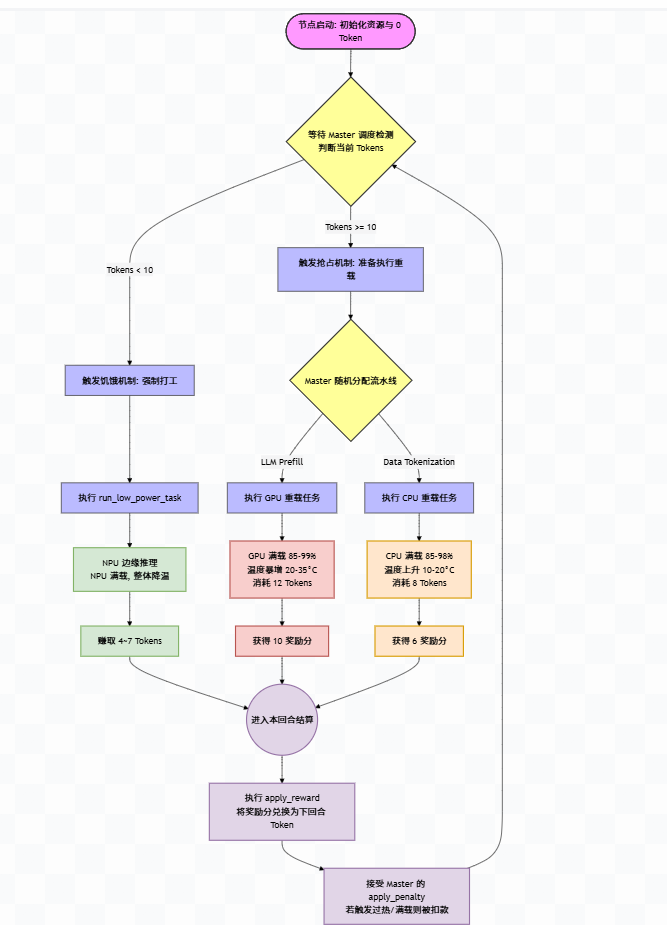
\includegraphics[width=0.8\textwidth]{agent1.png} % 设置图片宽度为正文宽度的 80%
    \caption{Worker agent 流程图} % 图片下方的标题
\end{figure}

\begin{figure}[htbp] %[htbp] 由 LaTeX 自动寻找最佳位置
    \centering
    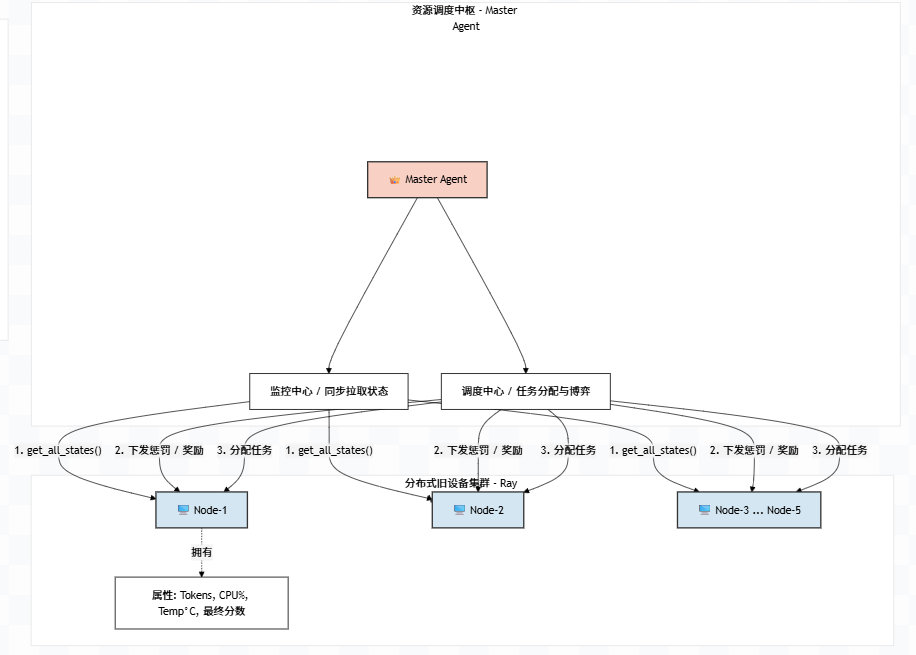
\includegraphics[width=0.8\textwidth]{agent2.png} % 设置图片宽度为正文宽度的 80%
    \caption{Master agent 流程图} % 图片下方的标题
\end{figure}

\section{实践中遇到的困难与解决办法}

\subsection{挑战 1：单机环境下的分布式调度与状态隔离}
\textbf{实践困难：} 在实验初期的代码编写阶段，首要难点是如何在单台个人笔记本电脑上，模拟出多台物理隔离的异构老旧设备并发运行，并对它们的状态进行统一、非阻塞的监控与追踪。传统的 Python 多线程/多进程库编写繁琐，且难以实现跨节点的对象状态同步。

\textbf{解决办法：} 放弃了底层并发库，选择引入成熟的 \textbf{Ray 框架} 实现分布式调度。通过将 \texttt{WorkerAgent} 类加上 \texttt{@ray.remote} 装饰器，直接将各设备实例化为 Ray 集群中独立的 Actor 进程。Master 节点只需通过远程方法调用（RPC）即可下发指令，并通过返回的对象引用（Object Ref）统一同步节点状态。

\begin{tcolorbox}[reflectionbox]
多 Agent 系统的设计精髓在于“去中心化的执行”与“中心化的监管”相分离。引入 Ray 框架不仅完美解决了本地进程隔离与异步通信的痛点，更为项目未来向真实的跨机器分布式集群平滑迁移奠定了基础。这种“单机模拟验证，无缝拓展至集群”的工程设计思维，是构建高可用分布式架构的最佳实践原则。
\end{tcolorbox}

\subsection{挑战 2：异构硬件特性的拟真与精细化资源博弈}
\textbf{实践困难：} 最初编写逻辑时，任务对资源的影响仅仅被粗暴地量化为单一的“CPU 占用”和“定值温度飙升”。这导致模拟结果过于刻板，不仅脱离了物理现实，也完全无法体现出现代 AI 大模型推理中 CPU、GPU、NPU 各自截然不同的功耗与发热特性，使得资源博弈失去了深度。

\textbf{解决办法：} 针对异构硬件进行多维度的状态拆解与随机化重构。我将节点状态拆分为独立的 CPU、GPU 和 NPU 占用率，并为大模型流水线上的不同环节设计了专属的资源指纹：GPU 负责的“LLM Prefill”不仅极度消耗 Token（12），还会导致温度剧烈飙升（增加 $20 \sim 35^\circ\text{C}$）；CPU 负责的“Data Tokenization”耗能与发热中等；而 NPU 则能在极低功耗下接管边缘推理赚取 Token，甚至实现物理降温。所有数值均使用 \texttt{random.uniform} 引入高斯噪声区间，以模拟真实物理环境的波动。

\begin{tcolorbox}[reflectionbox]
真实物理硬件的瓶颈往往是非线性的黑盒。将死板的单一变量改为多维度的异构“噪声区间”，彻底激活了博弈生态的复杂性。更重要的是，基于硬件异构特性，我将 Master 的“一刀切罚款”升级为了“阶梯式惩罚”（整体过热扣 15 分，GPU 撞墙扣 10 分，CPU 满载扣 5 分）。这种底层的“物理不可靠性”与精细化调控，使得 Master Agent 的调度策略面临更真实的博弈考验，完美模拟了现代系统应对硬件“过热降频（Thermal Throttling）”时的断臂求生机制。
\end{tcolorbox}

\subsection{挑战 3：回合制状态同步与异步执行的时序冲突}
\textbf{实践困难：} 随着模拟环境加入了随机耗时，不同进程的 Worker 节点任务执行步调产生差异。由于代码是异步调用的，导致 Master 在回合末尾拉取状态时发生了严重的“时序错位”——可能取到了上一回合尚未更新的旧数据。结算日志呈现出状态混乱，导致惩罚与奖励的逻辑判断发生误判，破坏了调度的公平性。

\textbf{解决办法：} 在 Master 的调度回合（Round）末尾，强制引入了时间与状态的“同步屏障”（Barrier）机制。在下发完所有异步任务后，首先使用 \texttt{time.sleep()} 让主进程短暂挂起等待执行完毕；最核心的改动是，在获取所有节点状态时，强制使用 \texttt{ray.get()} 的阻塞特性，确保所有 Actor 的远程状态均已正确更新并返回后，再打印本回合结算面板，随后进入下一轮的博弈。

\begin{tcolorbox}[reflectionbox]
这是分布式系统中经典的“一致性与并发性”冲突。在追求 Agent 并发执行效率的同时，必须在关键的业务节点（即本系统的每一回合结算点）建立强约束的“状态快照”。采用 \texttt{ray.get()} 阻塞拉取，虽然牺牲了极少量的主进程等待时间，却换来了整个博弈系统在逻辑调度上的绝对一致性与正确性。若无状态的一致性保证，基于此产生的所有 Token 扣除和奖励都将失去合法依据。在特定环节“以局部同步保全局一致”，是复杂调度系统不可或缺的设计妥协。
\end{tcolorbox}

\section{不足与观察思考}

\begin{tcolorbox}[reflectionbox]
\textbf{物理约束的巧妙投射：}
实验证明，在这个多 Agent 系统中，“电费 Token”本质上起到了系统“热量缓冲池（Thermal Headroom）”的作用。传统的纯算力调度容易把边缘机器烧毁，而我们利用 Token 作为惩罚介质，一旦 GPU 触发温度墙，立刻剥夺其高负载权限，强制将其切换到 NPU 避险。这完美复刻了现代硬件底层的过热降频（Thermal Throttling）机制，是一种高度安全且健壮的调度范式。

\textbf{现存不足与未来改进方向：}
目前的阶梯式惩罚（扣 15/10/5 分）仍偏向于硬编码。真实操作系统的资源调度器（如 Linux 的 CPUFreq）使用的是平滑的 PID 控制或动态电压频率调整（DVFS）。未来可以引入大模型进行更微观的预测性调度，不仅监控温度，还应将大模型推理过程中极为重要的 \textbf{KV Cache（显存占用）} 纳入状态向量，使节点资源的博弈维度更加完善。
\end{tcolorbox}

\renewcommand{\refname}{参考文献}

\begin{thebibliography}{99}

% 1. 关于大模型推理资源调度与显存管理 (GPU) 的顶会论文 (vLLM 的出处)
\bibitem{kwon2023vllm}
Kwon, W., Li, Z., Zhuang, S., Sheng, Y., Zheng, L., Yu, C. H., ... \& Stoica, I. (2023). 
\textit{Efficient memory management for large language model serving with pagedattention}. 
In \textit{Proceedings of the 29th Symposium on Operating Systems Principles} (SOSP 2023, pp. 611-626).

% 2. 关于基于 LLM 的多智能体 (Multi-Agent) 系统的最新权威综述
\bibitem{wang2024agent}
Wang, L., Ma, C., Feng, X., Zhang, Z., Yang, H., ... \& Ji, H. (2024). 
\textit{A survey on large language model based autonomous agents}. 
\textit{Frontiers of Computer Science}, 18(6), 1-26.

% 3. 关于边缘计算/异构硬件 (NPU/GPU) 上进行大语言模型低功耗加速的研究
\bibitem{lin2023awq}
Lin, J., Tang, J., Tang, H., Yang, S., Dang, X., \& Han, S. (2023). 
\textit{AWQ: Activation-aware Weight Quantization for LLM Compression and Acceleration}. 
In \textit{Proceedings of Machine Learning and Systems} (MLSys 2024).

% 4. 关于分布式深度学习系统自动切分与调度的顶会论文 (可作为 Ray 场景的补充补充)
\bibitem{zheng2022alpa}
Zheng, L., Li, Z., Zhang, H., Zhuang, S., Gonzalez, J. E., \& Stoica, I. (2022). 
\textit{Alpa: Automating inter-and intra-operator parallelism for distributed deep learning}. 
In \textit{16th USENIX Symposium on Operating Systems Design and Implementation} (OSDI 2022, pp. 559-578).

% 5. 引用你在报告中提到的 LangChain 工具 (软件/框架引用规范)
\bibitem{chase2023langchain}
Chase, H. (2023). 
\textit{LangChain: Building applications with LLMs through composability}. 
GitHub repository. \url{https://github.com/langchain-ai/langchain}

\end{thebibliography}

\appendix
\section{附录:github链接}
\begin{itemize}
    \item \textbf{项目代码仓库}：\url{https://github.com/jiling-shenyi/Shujutongxing}
\end{itemize}
\section{附录:实验结果}
\begin{figure}[htbp]
\centering
\subfigure[1-2]
{
    \begin{minipage}[b]{.4\linewidth}
        \centering
        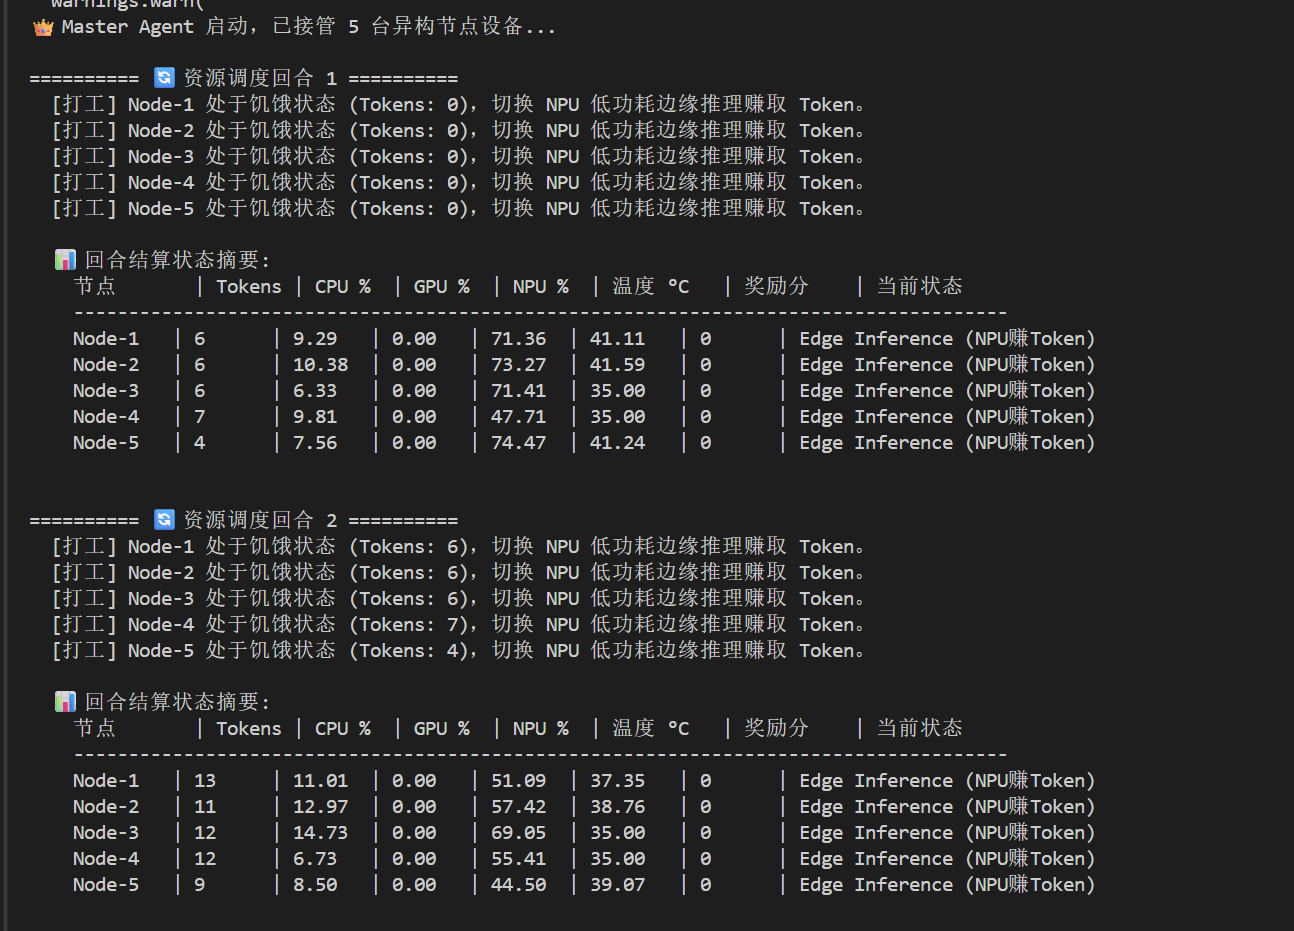
\includegraphics[scale=0.3]{1-2.png}
    \end{minipage}
}
\subfigure[3-4]
{
 	\begin{minipage}[b]{.4\linewidth}
        \centering
        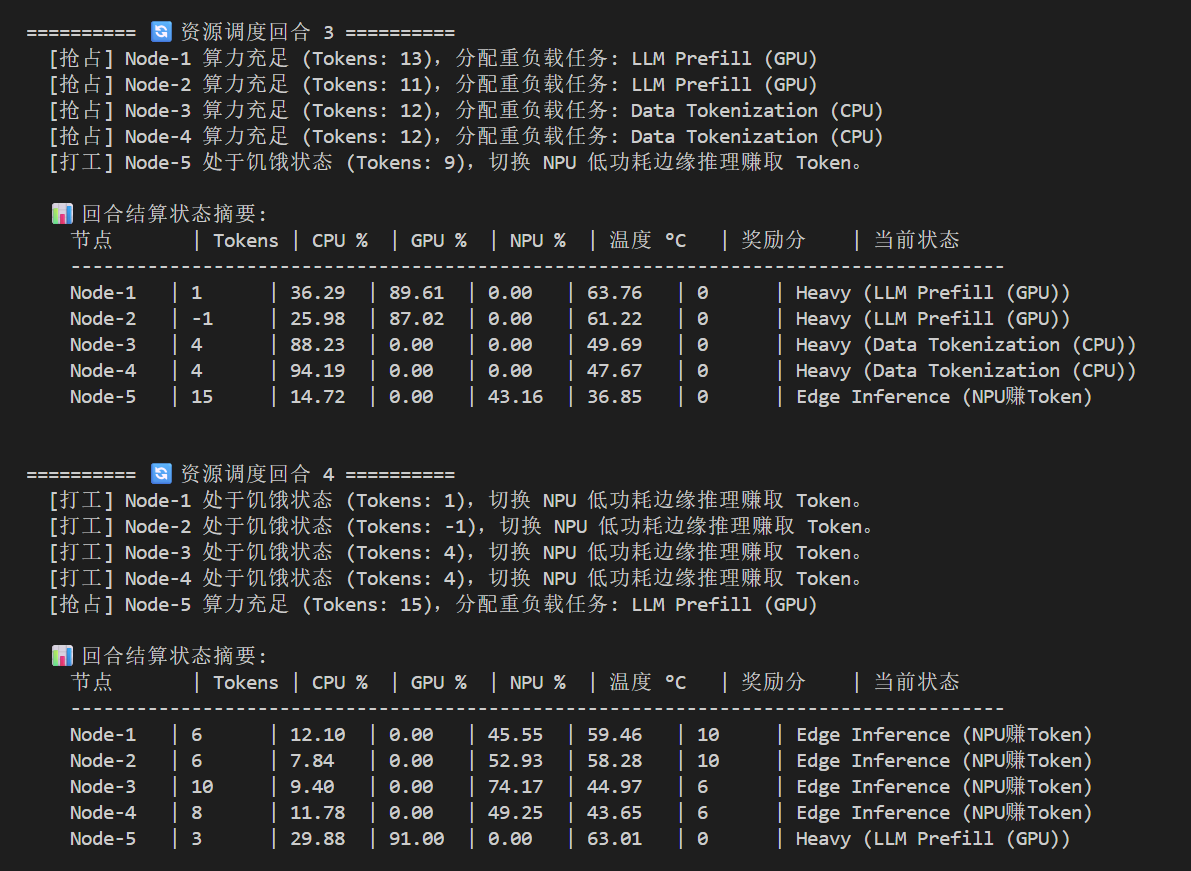
\includegraphics[scale=0.3]{3-4.png}
    \end{minipage}
}
\caption{1-4回合}
\end{figure}

\begin{figure}[htbp]
\centering
\subfigure[5-6]
{
    \begin{minipage}[b]{.4\linewidth}
        \centering
        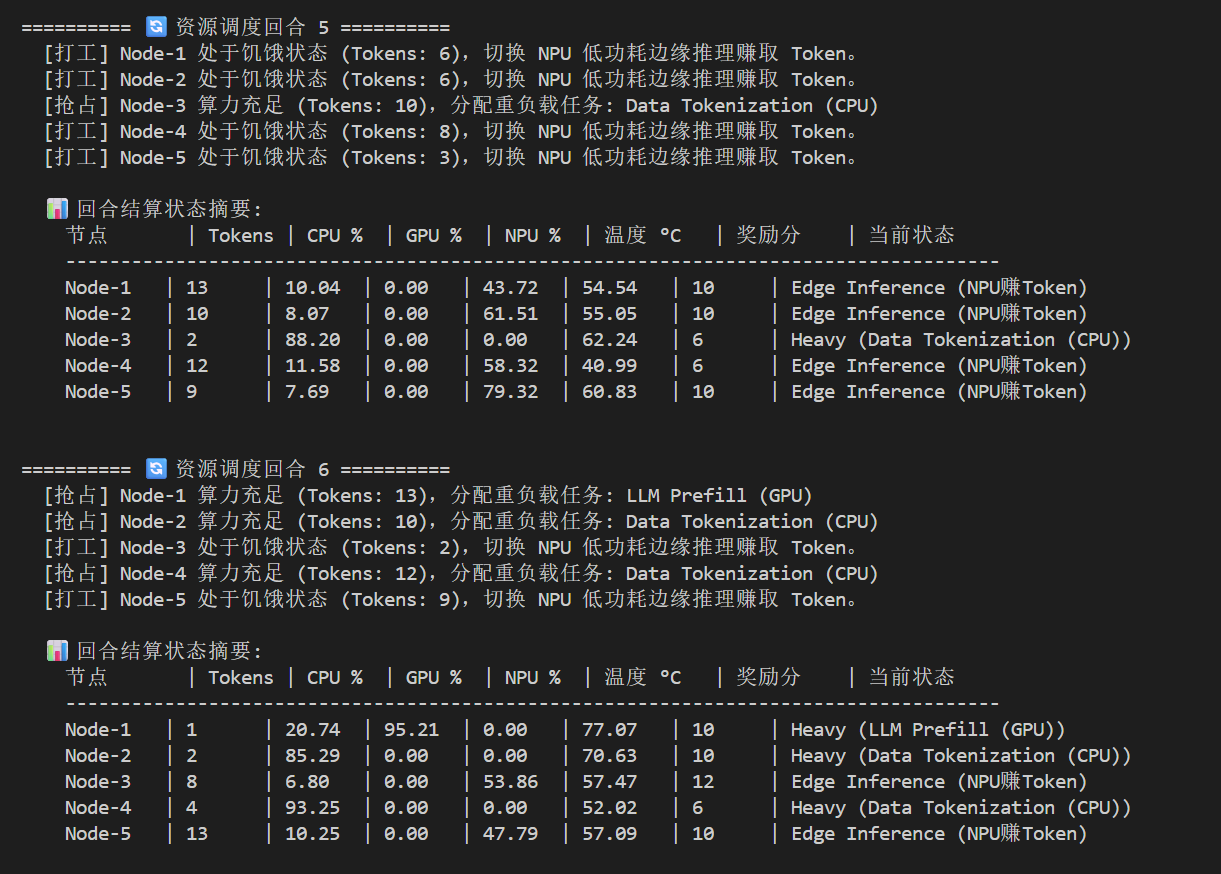
\includegraphics[scale=0.3]{5-6.png}
    \end{minipage}
}
\subfigure[7-8]
{
 	\begin{minipage}[b]{.4\linewidth}
        \centering
        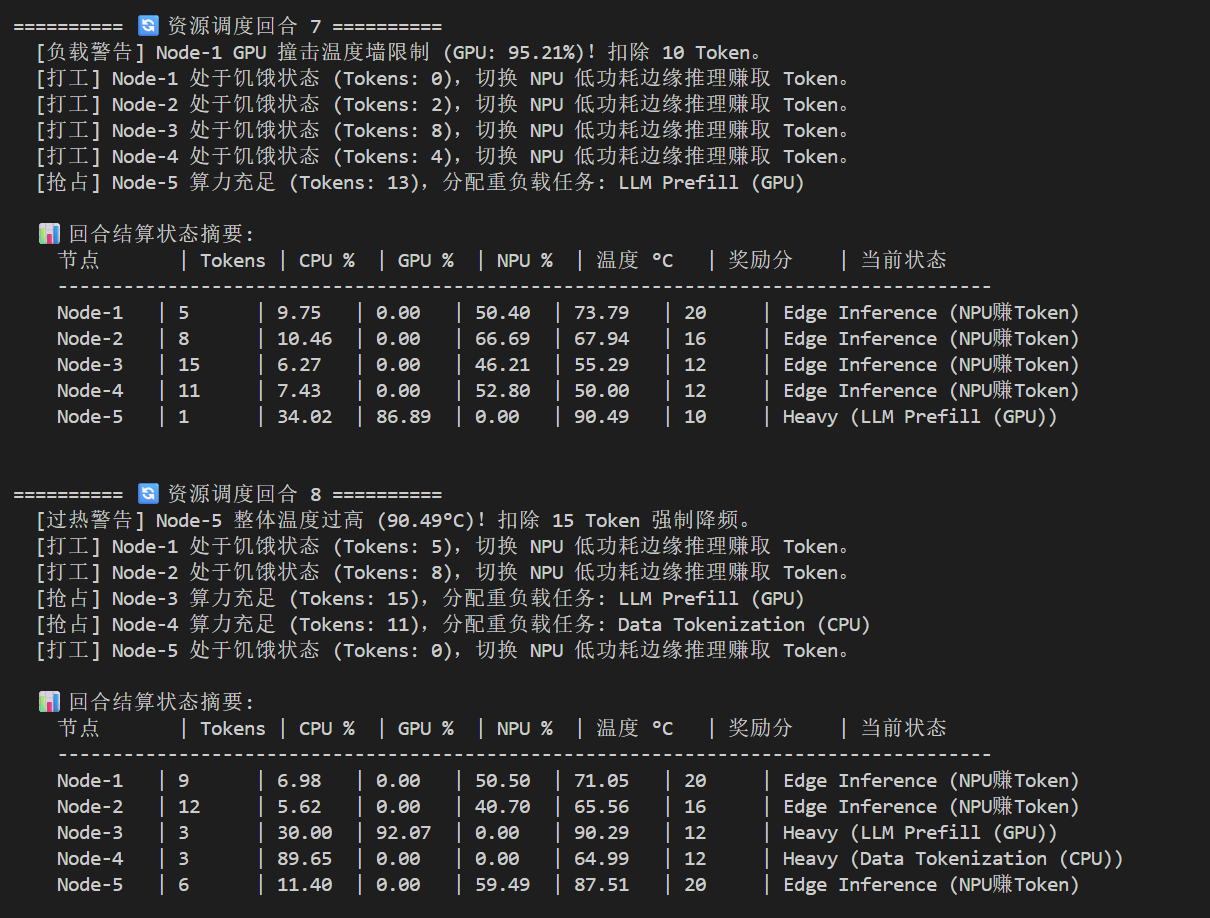
\includegraphics[scale=0.3]{7-8.png}
    \end{minipage}
}
\caption{5-8回合}
\end{figure}

\begin{figure}[htbp]
\centering
\subfigure[9-10]
{
 	\begin{minipage}[b]{.4\linewidth}
        \centering
        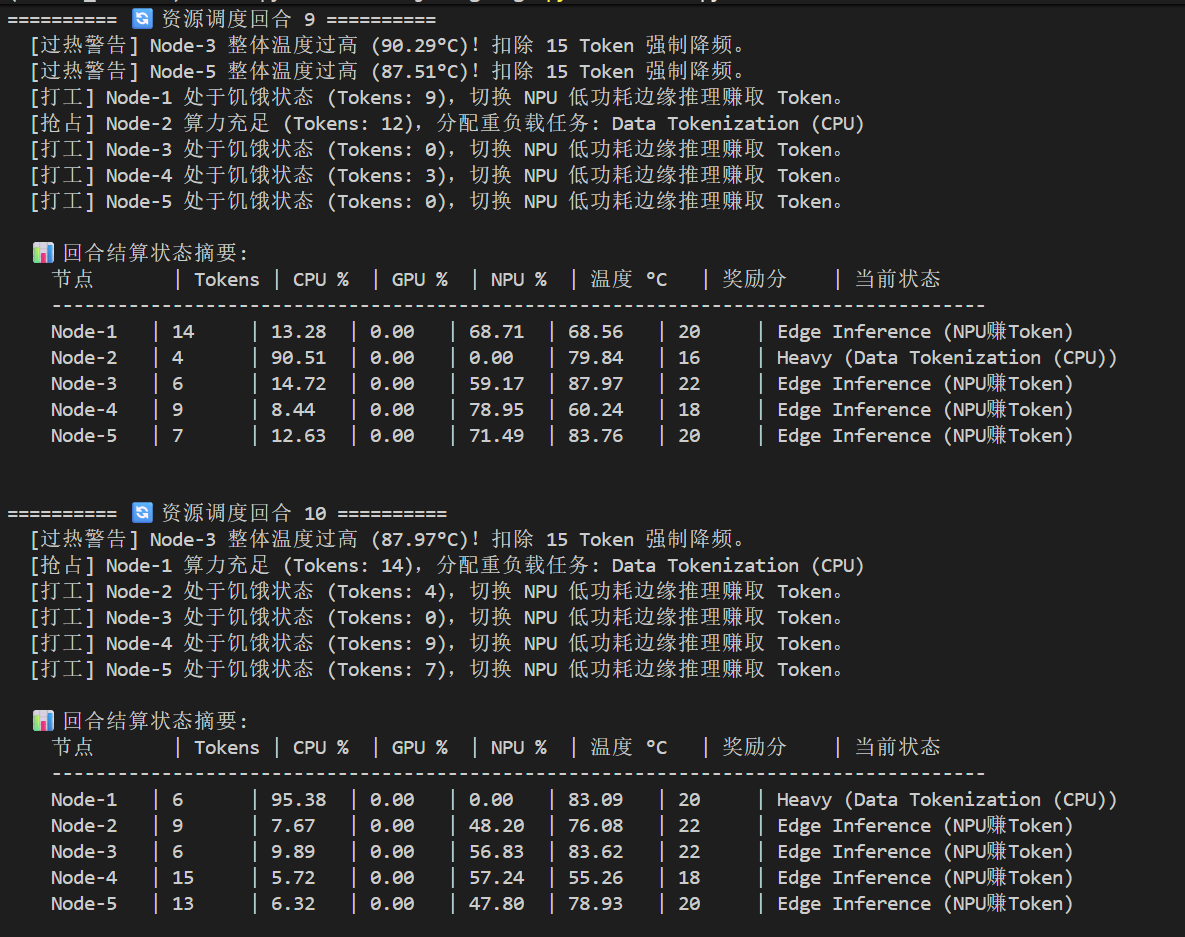
\includegraphics[scale=0.4]{9-10.png}
    \end{minipage}
}
\caption{9-10回合}
\end{figure}

\end{document}